\documentclass[12pt,onecolumn,a4paper]{article}
\usepackage{epsfig,graphicx,subfigure,amsthm,amsmath, amssymb}
\usepackage{color,xcolor}     
\usepackage{xepersian}
\settextfont[Scale=1]{sahel.ttf}
\setlatintextfont[Scale=1]{Times New Roman}
\graphicspath{ {./img/} }


\begin{document}


\title{گزیده و نکات بخش سوم، احتمال\\\lr{"Introductory Statistics" by Wonnacott}} 
\author{مهدی صادق‌زاده قمصری}
\date{بهمن ۹۹}
\maketitle

\section{تعریف احتمال\footnote{\lr{probability}}} 
احتمال را برابر میزان تکرار، نسبت به تعداد آزمایش ها در حد بی‌نهایت تعریف می‌کنند؛ یا به عبارت دیگر تکرار نسبی در حد بی نهایت:
\begin{equation}
    Pr(\text{\lr{$e$}}_1) \triangleq \lim_{n \rightarrow \infty} {\dfrac{n_1}{n}}
\end{equation}
تعاریف دیگری هم برای احتمال وجود دارد اما این تعریف شهود بهتری می‌دهد. درباره سایر دیدگاه ها در مورد تعریف احتمال، در اخر بخش مطالبی مطرح شده.

\section{ویژگی های احتمال}
\begin{itemize}
    \item تکرار رخداد ها هیچ‌گاه منفی نخواهد بود. نتیجتا:
        \begin{equation}
            Pr(\text{\lr{$e$}}_i) \geq 0
        \end{equation}
    \item داریم:
        \begin{align*}
            n_1 + n_2 + ... + n_N = n \\
            \Rightarrow \dfrac{n_1}{n} + \dfrac{n_2}{n} + ... + \dfrac{n_N}{n} = 1
        \end{align*}
        \begin{equation}
            \Rightarrow Pr(\text{\lr{$e$}}_1) + Pr(\text{\lr{$e$}}_2) + ... + Pr(\text{\lr{$e$}}_N) = 1
        \end{equation}
    \item معادلات ۲ و ۳ نتیجه می‌دهند:
        \begin{equation}
            Pr(\text{\lr{$e$}}_i) \leq 1
        \end{equation}
\end{itemize}

\section{رخدادها و احتمالات آنها}
\begin{itemize}
    \item مجموعه حالات\footnote{\lr{outcome set}}(برآمد ها): 
        به مجموعه کل برآمد\footnote{\lr{outcome}} های یک نمونه، گفته می شود.
    \item رخداد\footnote{\lr{event}}: یک رخداد زیرمجموعه ای از مجموعه حالات است. احتمال هر رخداد به شکل زیر محاسبه می‌شود:
        \begin{align*}
            Pr(E) &= \lim_{n\rightarrow\infty}{\dfrac{n_E}{n}} \\
            &= \lim(\dfrac{n_1}{n}+\dfrac{n_2}{n}+...+\dfrac{n_k}{n}) \\
            &= Pr(\text{\lr{$e$}}_1)+Pr(\text{\lr{$e$}}_2)+...+Pr(\text{\lr{$e$}}_k) 
        \end{align*}
        \begin{equation}
            \Rightarrow Pr(E) = \sum Pr(\text{\lr{$e$}}_i)
        \end{equation}
    \item ترکیب رخدادها: \\ 
        همان قوانین مجموعه ها درباره رخدادها هم برقرار است:
        \begin{equation}
            Pr(G\cup H)=Pr(G)+Pr(H)-Pr(G\cap H)
        \end{equation}
         \begin{equation}
            Pr(\bar{E}) = 1 - Pr(E) 
         \end{equation}
\end{itemize}

\section{احتمال شرطی}
احتمال شرطی را می‌توان به این صورت بیان کرد: در صورتی که رخداد \lr{G} رخ داده باشد؛ احتمال روی‌دادن رخداد \lr{H} را احتمال شرطی روی‌دادن \lr{H | G} می‌گوییم.

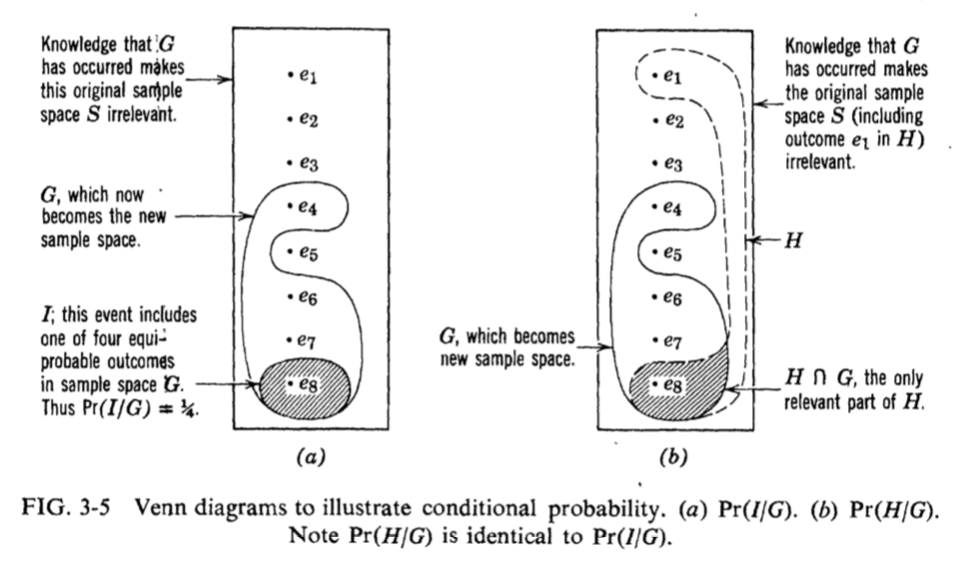
\includegraphics[width=\textwidth]{fig1.png} \\

همانطور که از شکل هم پیداست، در صورتی که \lr{G} رخ داده باشد؛ برآمد هایی میتواند رخ دهد تنها به برآمد های موجود در \lr{G} خلاصه می‌شود. 
نتیجتا تعداد تکرار برآمد های رخداد \lr{H} به شرط \lr{G} را می‌توان به عنوان \lr{n(H|G)} در نظر داشت. مجموعه کل برآمد ها نیز در این حالت همان \lr{G} است(نه کل مجموعه حالات، زیرا رخداد \lr{G} رخ داده است) پس داریم:
\begin{align*}
    Pr(H|G) &\triangleq \lim_{n\rightarrow\infty} {\dfrac{n(H\cap G)}{n(G)}} \\
    &= \dfrac{\lim_{n\rightarrow\infty}{\dfrac{n(H\cap G)}{n}}} {\lim_{n\rightarrow\infty}{\dfrac{n(G)}{n}}}
\end{align*}
\begin{equation}
     \Rightarrow Pr(H|G) = \dfrac{Pr(H\cap G)}{Pr(G)}
\end{equation}


\section{استقلال}
دو رخداد نسبت به یکدیگر از لحاظ آماری مستقل\footnote{\lr{independent}} محسوب می‌شوند اگر و تنها اگر:
\begin{equation}
    Pr(E|F) = Pr(E)
\end{equation}
عکس این معادله نیز به سادگی با توجه به معادله ۸ ثابت می‌شود.

\section{دیدگاه های دیگر به احتمال}
با رویکرد های دیگری نیز می‌توان به احتمال پرداخت:
\begin{itemize}
    \item احتمال متقارن(\lr{Symmetric Probability}) \\
        با این نگاه احتمال به شکل زیر تعریف می‌شود:
        \begin{equation}
            Pr(E) = \dfrac{N_E}{N}
        \end{equation}
        این تعریف تنها در حالتی اثبات می‌شود که فرض کنیم همه برآمد ها با یکدیگر معادل اند و در صورتی که این برابری برقرار نباشد، این نگاه نمی‌تواند نظری داشته باشد. جدای از این موضوع، ذات برابری برآمدها نوعی خود به تعریف احتمال برمیگردد؛ که این چرخه در استدلال را می‌توان ضعف فلسفی این نگاه دانست. \\
        مبنا قرار دادن تکرار نسبی در تعریف ما از احتمال(معادله ۱) نیز مشکل مشابهی دارد؛ زیرا این فرض که در تعداد زیادی آزمایش به احتمال واقعی نزدیک‌تر می‌شویم، خود نوعی تعریف احتمال است.
    \item اصول موضوعه احتمال(\lr{Axiomatic Objective Probability}) \\
        در این نگاه، اصل\footnote{\lr{axiom}} های زیر در نظر گرفته می‌شوند:
        \begin{align*}
            Pr(\text{\lr{$e$}}_i) \geq 0 \\
            Pr(\text{\lr{$e$}}_1) + ... + Pr(\text{\lr{$e$}}_N) = 1 \\
            Pr(E) = \sum Pr(\text{\lr{$e$}}_i)
        \end{align*}
        و سایر معادلات بر اساس این اصول اثبات می‌شوند؛ مانند معادله ۱ و ۴ و ۷ و ... \\
        معادله ۱ به طور خاص اهمیت زیادی دارد و به عنوان قانون اعداد بزرگ شناخته می‌شود(کجا ها استفاده میشه؟).
    \item \lr{Subjective Probability} \\ 
        بعضا به آن احتمال شخصی هم گفته می‌شود؛ در اصل این نگاه برای پاسخ به نیاز تخمین درباره حالات مختلف رخداد هایی به وجود آمده است که تکرار نمی‌شوند. در بخش ۱۵ استفاده این نگاه در نظریه تصمیم\footnote{\lr{decision theory}} را خواهیم‌دید.
\end{itemize}

\end{document}